% Standalone TikZ source for Figure 1 (fig_cascade.pdf).
% Compile separately:  tectonic fig_cascade.tex  -> produces fig_cascade.pdf
\documentclass[tikz,border=4pt]{standalone}
\usetikzlibrary{positioning,arrows.meta,shapes.geometric,fit,calc}

\begin{document}
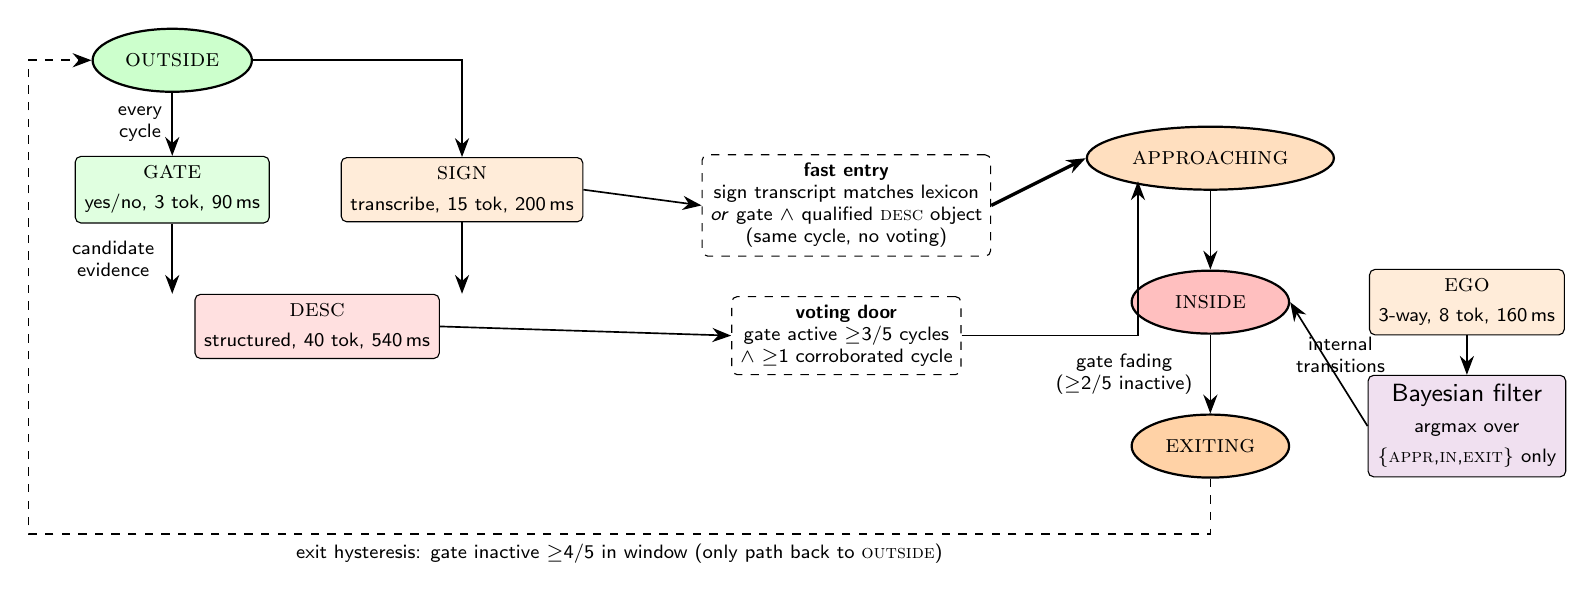
\begin{tikzpicture}[
  font=\small\sffamily,
  node distance=6mm and 9mm,
  chan/.style={draw, rounded corners=2pt, minimum height=7mm, minimum width=21mm, align=center, fill=blue!8},
  cheap/.style={chan, fill=green!12},
  mid/.style={chan, fill=orange!15},
  costly/.style={chan, fill=red!12},
  state/.style={draw, ellipse, minimum height=8mm, minimum width=20mm, align=center, thick},
  arr/.style={-{Stealth[length=2.4mm]}, semithick},
  lab/.style={font=\scriptsize\sffamily, align=center},
  door/.style={draw, rounded corners=2pt, dashed, align=center, font=\scriptsize\sffamily, inner sep=3pt}
]

% ---------------- OUTSIDE patrol column ----------------
\node[state, fill=green!20] (outside) {\textsc{outside}};

\node[cheap, below=8mm of outside] (gate) {\textsc{gate}\\\scriptsize yes/no, 3 tok, 90\,ms};
\node[mid, right=of gate] (sign) {\textsc{sign}\\\scriptsize transcribe, 15 tok, 200\,ms};
\node[costly, below=9mm of $(gate.south)!0.5!(sign.south)$] (desc) {\textsc{desc}\\\scriptsize structured, 40 tok, 540\,ms};

\draw[arr] (outside) -- node[lab, left] {every\\cycle} (gate);
\draw[arr] (outside) -| (sign);
\draw[arr] (gate.south) -- node[lab, left, xshift=-1mm] {candidate\\evidence} (desc.north -| gate.south);
\draw[arr] (sign.south) -- (desc.north -| sign.south);

% ---------------- entry doors ----------------
\node[door, right=15mm of sign, yshift=-2mm] (fast) {\textbf{fast entry}\\sign transcript matches lexicon\\\emph{or} gate $\wedge$ qualified \textsc{desc} object\\(same cycle, no voting)};
\node[door, below=5mm of fast] (vote) {\textbf{voting door}\\gate active $\geq$3/5 cycles\\$\wedge \geq$1 corroborated cycle};

\draw[arr] (sign.east) -- (fast.west);
\draw[arr] (desc.east) -- (vote.west);

% ---------------- ACTIVE side ----------------
\node[state, fill=orange!25, right=12mm of fast, yshift=6mm] (appr) {\textsc{approaching}};
\node[state, fill=red!25, below=10mm of appr] (inside) {\textsc{inside}};
\node[state, fill=orange!35, below=10mm of inside] (exiting) {\textsc{exiting}};

\draw[arr, very thick] (fast.east) -- (appr.west);
\draw[arr] (vote.east) -| ($(appr.south west)+(2mm,0)$);

% ego + bayes
\node[mid, right=10mm of inside] (ego) {\textsc{ego}\\\scriptsize 3-way, 8 tok, 160\,ms};
\node[chan, below=5mm of ego, fill=violet!12] (bayes) {Bayesian filter\\\scriptsize argmax over\\\scriptsize \{\textsc{appr},\textsc{in},\textsc{exit}\} only};
\draw[arr] (ego) -- (bayes);
\draw[arr] (bayes.west) -- node[lab, above, pos=0.35] {internal\\transitions} (inside.east);

% internal transitions between active states
\draw[arr] (appr) -- (inside);
\draw[arr] (inside) -- node[lab, left, xshift=-1mm] {gate fading\\($\geq$2/5 inactive)} (exiting);

% exit hysteresis back to outside: routed BELOW all nodes to avoid overlaps
\coordinate (botL) at ($(outside.west)+(-8mm,0)$);
\draw[arr, dashed]
   (exiting.south) -- ++(0,-7mm)
   -| node[lab, below, pos=0.25]
        {exit hysteresis: gate inactive $\geq$4/5 in window (only path back to \textsc{outside})}
      (botL |- exiting)
   -- (botL)
   -- (outside.west);

\end{tikzpicture}
\end{document}
